\section{System's Perspective}
\label{sec:systems_perspective}

\subsection{Overview}
\label{subsec:systems_perspective_overview}
The initial project was a full stack \textit{Flask} application written in \textit{Bash} and \textit{Python2} with an \textit{SQLite} database. 
This implementation (henceforth referenced as \mini) included refactoring the initial project to the following containerized microservices:
\begin{itemize}
    \item \textit{\cs}backend using the \textit{ASP.NET Core web framework} and \textit{EF Core} object-relational mapping.
    \item \textit{ReactJS} single-page application frontend.
    \item \textit{PostgreSQL} database.
\end{itemize}
Upon which a monitoring stack and temporarily a logging stack were added to be served as a containerized application behind a load-balancer on a managed \textit{Kubernetes} cluster (\textit{DOKS})

\subsection{System Design}
\label{subsec:system_design}
The following section discusses our system design by supplying diagrams to illustrate the designs.
The backend, which decomposition can be seen in Figure \ref{fig:decompositionBackend}, is the most crucial part of the system as this is the part that contains our logic and API endpoints for the simulation.
Some files have been excluded from the diagram to simplify it.
These files include Dockerfiles, App settings files, and the program.cs file, which is the system's entry point, a legacy controller, and its interface for the frontend, which is now only used in tests.

\begin{figure}[H]
    \centering
    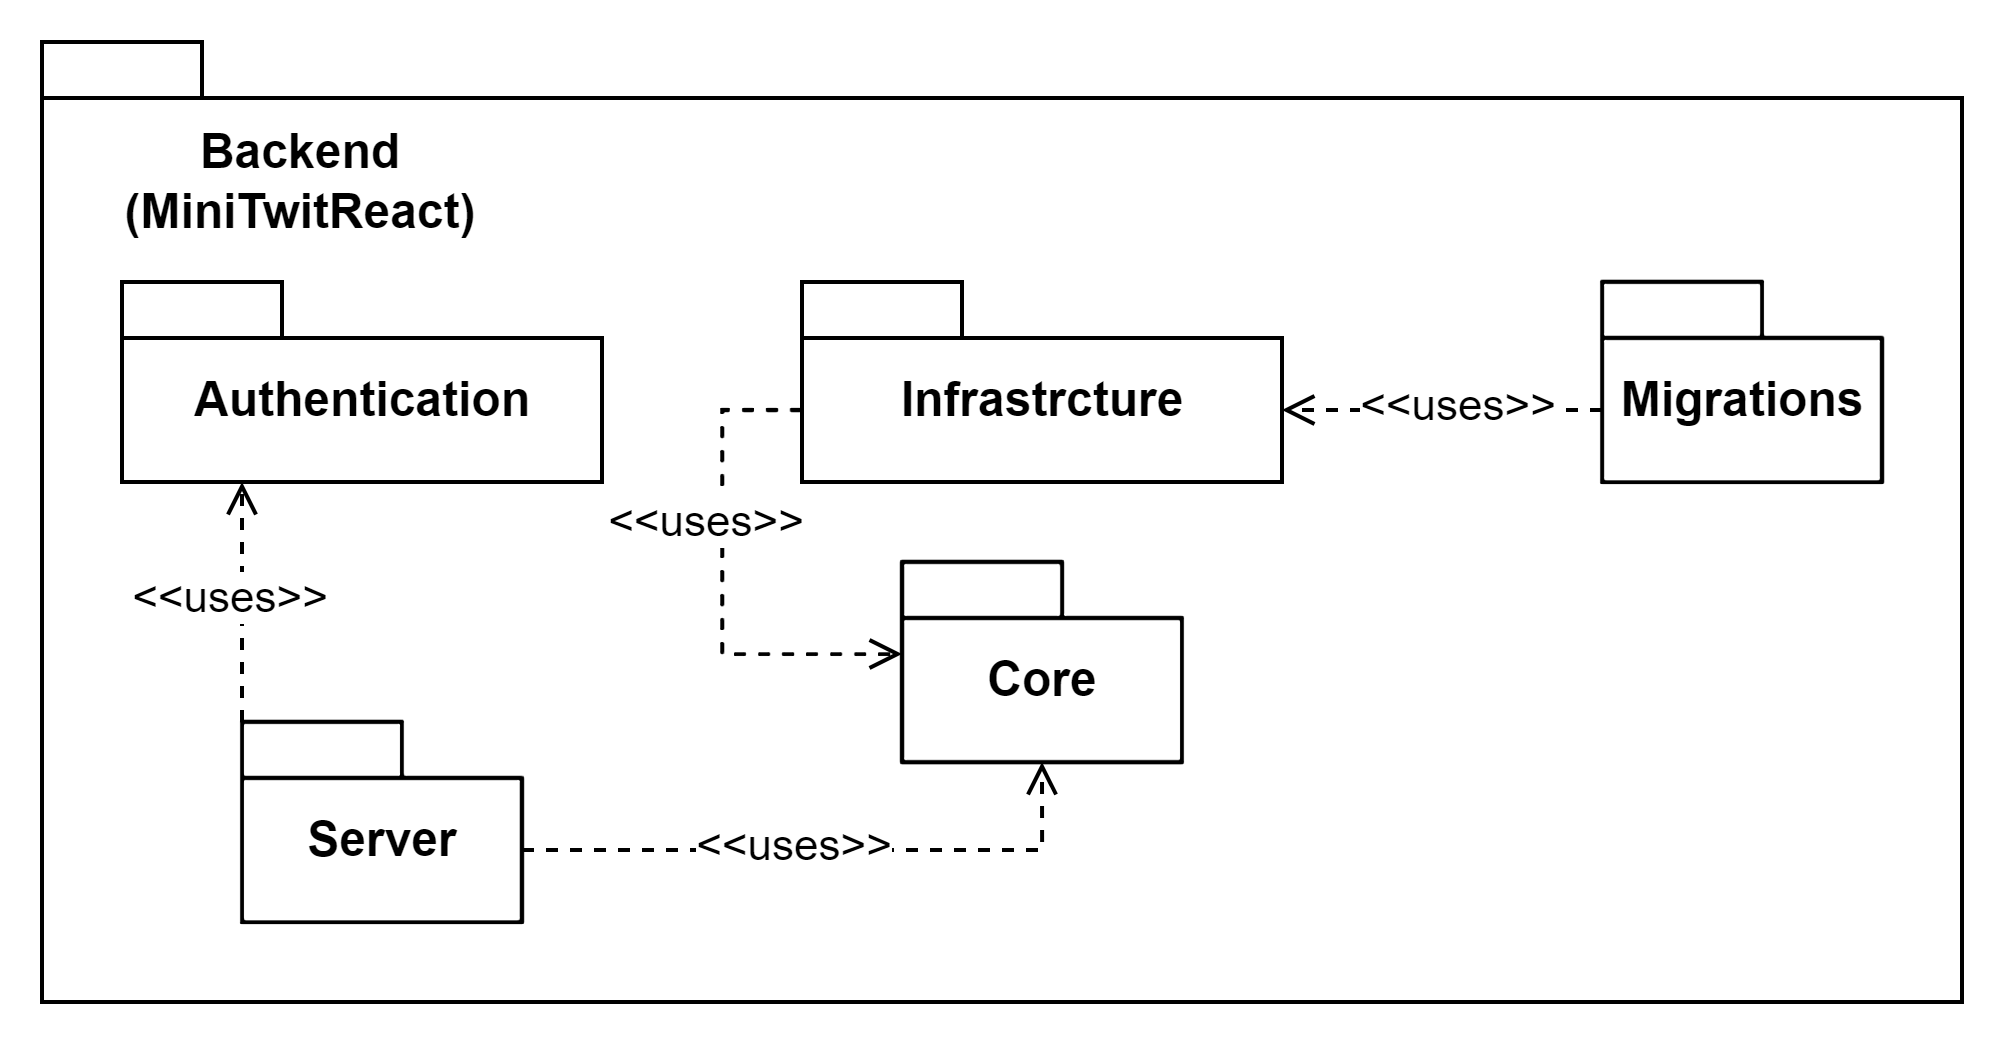
\includegraphics[scale=0.18]{images/package_class-diagrams/decomposition_backend.png}
    \caption{Decomposition of Backend Package of the \mini System}
    \label{fig:decompositionBackend}
\end{figure}


When we refactored the system, we decided to change the architecture to follow The Clean Architecture guidelines, introduced by Robert C. Martin \cite{clean}. We wanted the codebase to be easier to maintain, test and scale; and, by that, avoid technical debt.
This is achieved by following The Dependency Rule \cite{clean}, which states that source code dependencies can only point inwards.

\begin{figure}[H]
    \centering
    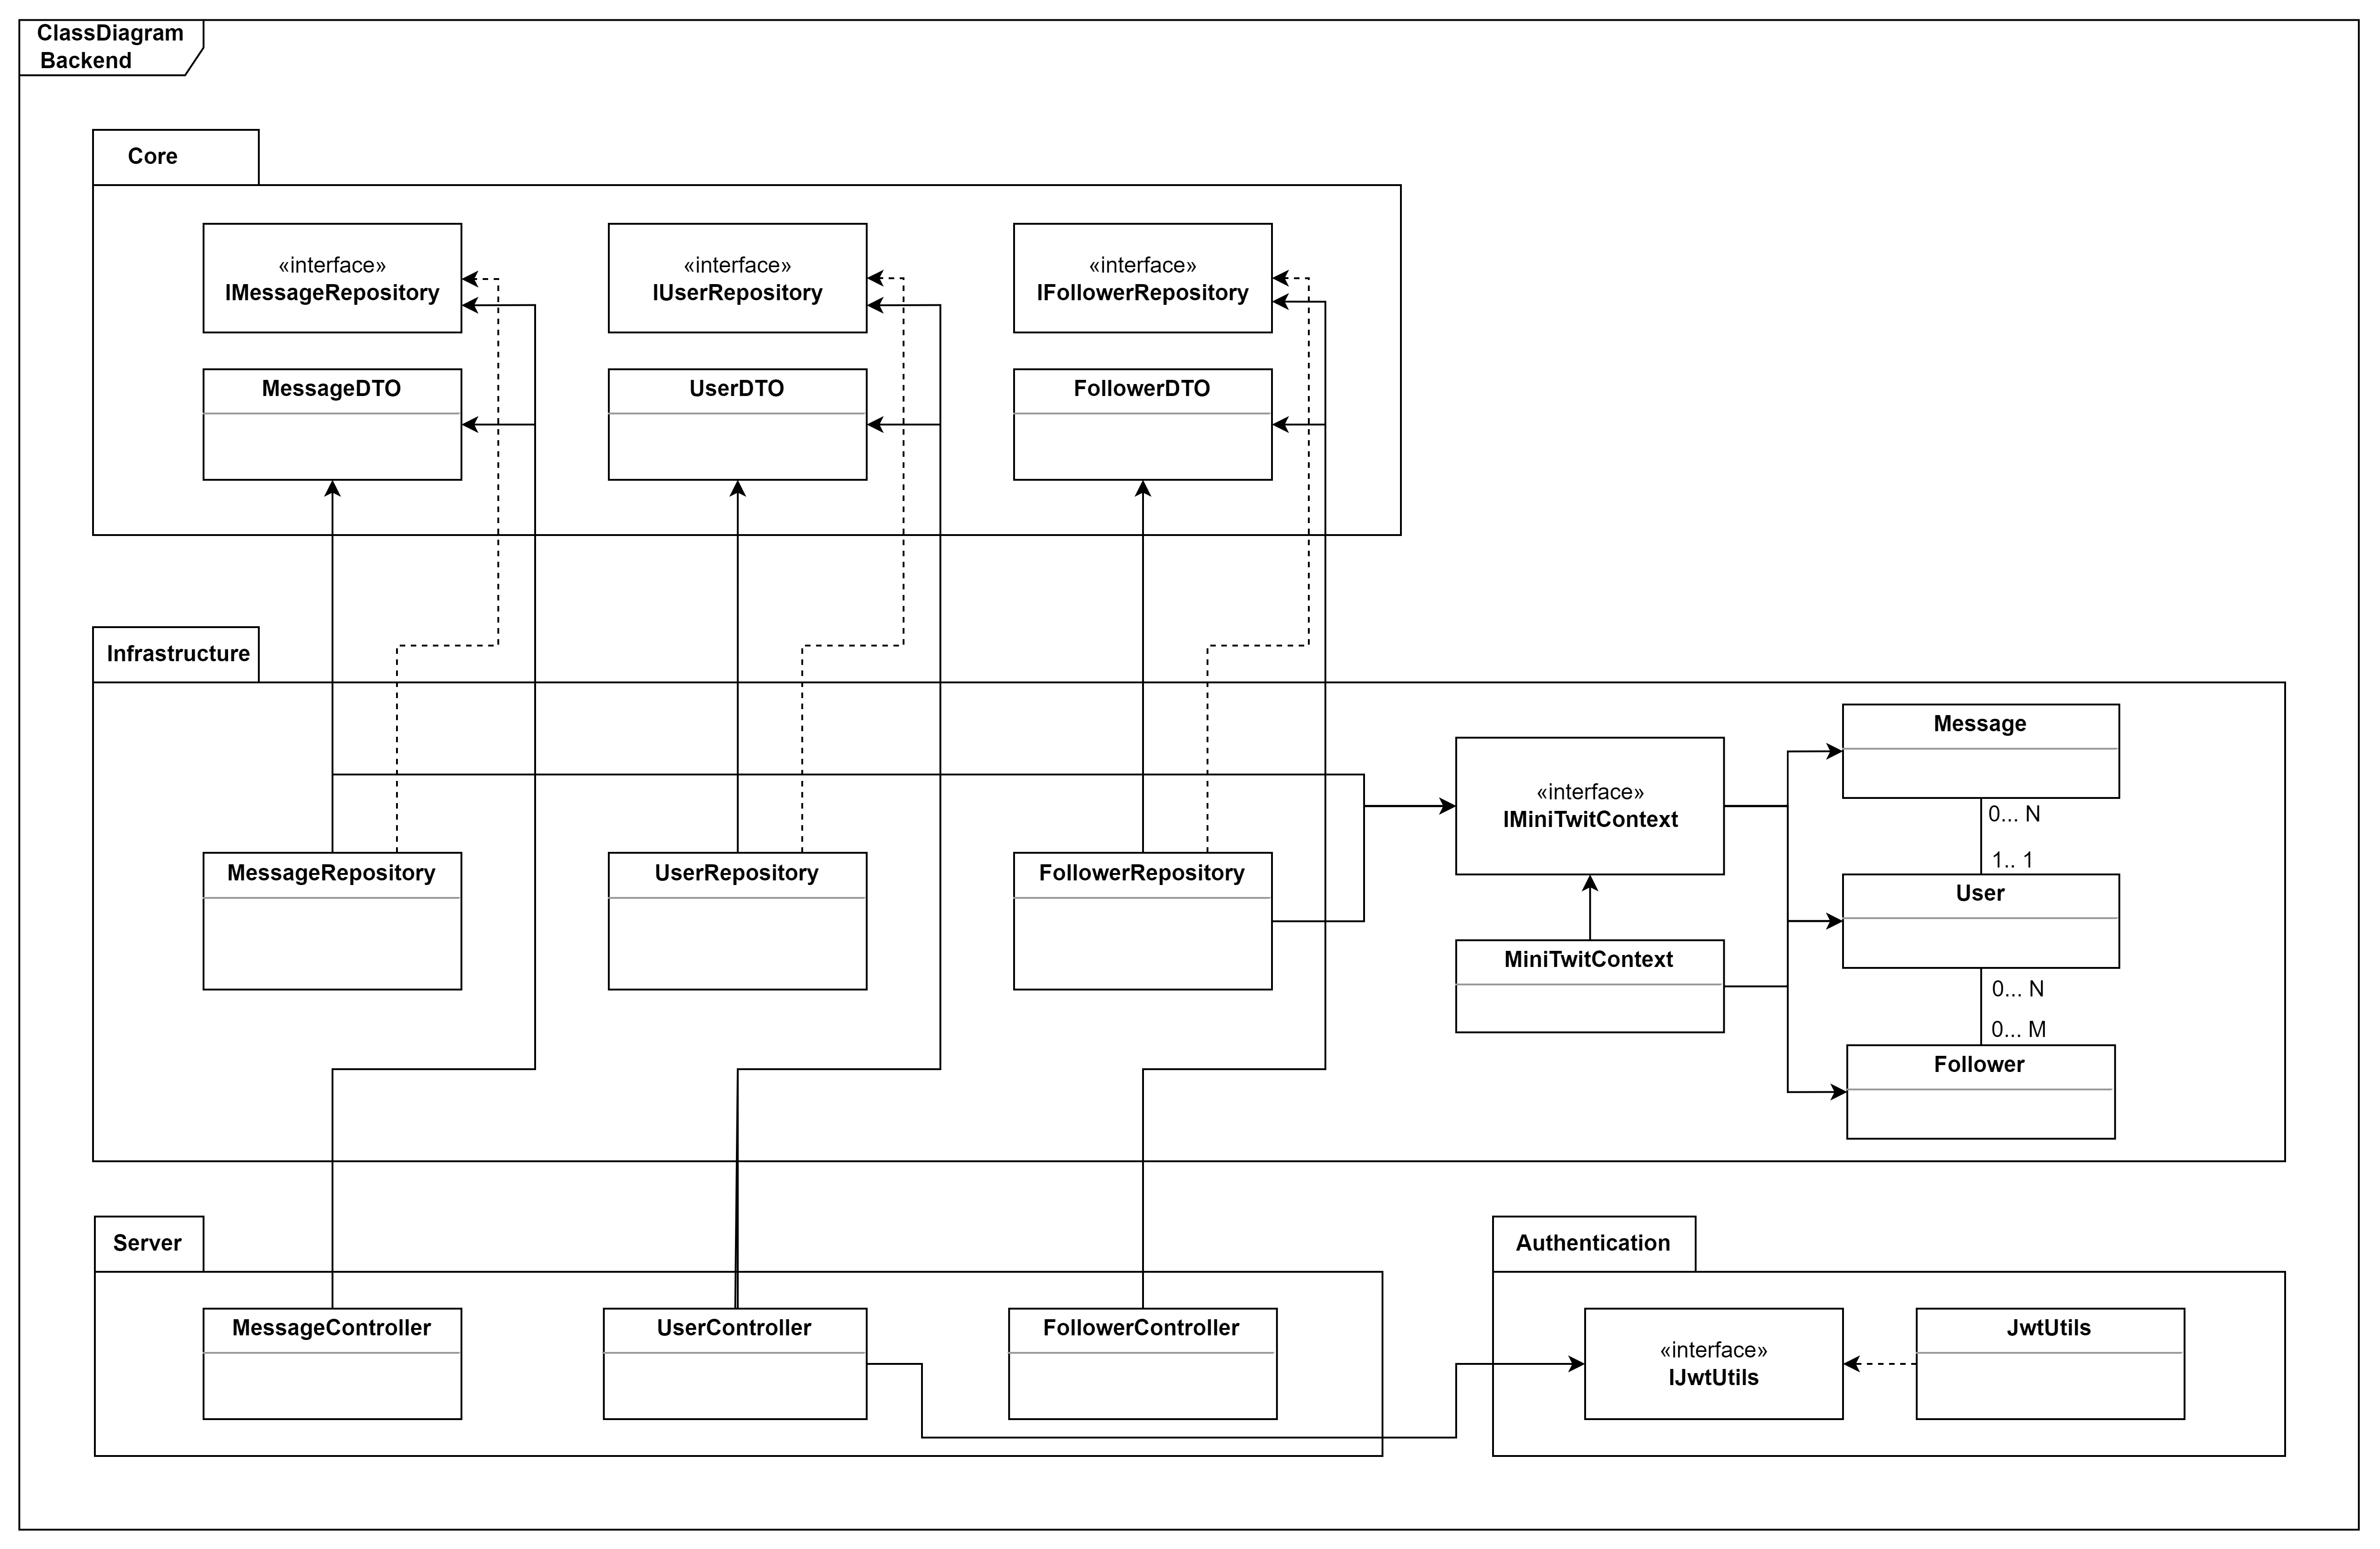
\includegraphics[scale=0.088]{images/package_class-diagrams/class_diagram_backend.png}
    \caption{Class Diagram Illustrating The Clean Architecture-pattern.}
    \label{fig:diagramClass}
\end{figure}

In figure \ref{fig:diagramClass} we can see the new refactored design: all dependencies point towards the core package, and each lower-level tier only have dependencies pointing towards a tier closer to this package. \\
Note that each entity has a separate implementation of the repository-DTO- and controller-class; this complies with the single responsibility principle. Additionally, we only depend on abstractions, i.e. the \texttt{UserController} depends on the \texttt{IUserRepository}, and not directly on the implementation of \texttt{UserRepository}. All these principles derive from the SOLID principles (also introduced by Martin).\\

The system consists of 5 containerized microservices (see Figure \ref{fig:microservices}).
One of these is the backend, which contains the business logic, provides two open APIs, an Object-Relational Mapping to our database, and exposes application-specific \textit{PromQL} metrics for \textit{Prometheus}. \par

\begin{figure}[H]
    \centering
    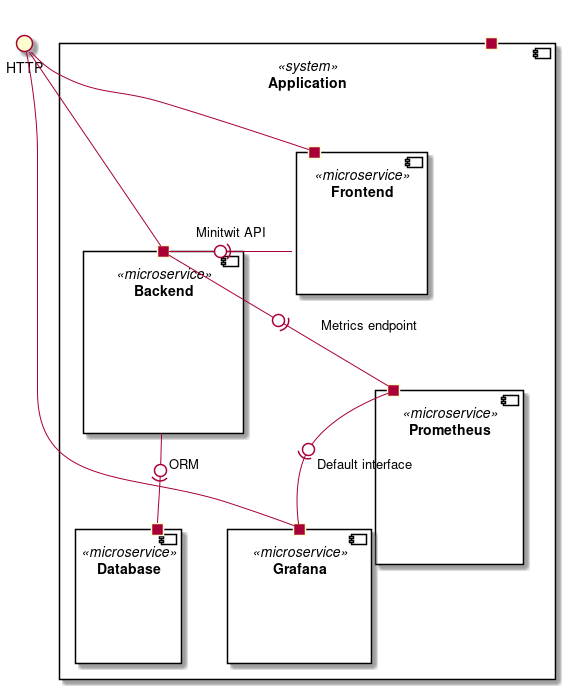
\includegraphics[scale=.43]{images/microservices-components.png}
    \caption{Component diagram of application microservices}
    \label{fig:microservices}
\end{figure}

This design pattern favors load balancing and horizontal scaling as most microservices serve a singular purpose and are non-critical to each other.

\subsection{System Architecture}
\label{subsec:system_architecture}
% - architecture of your itu-minitwit systems
% - all dependencies of your itu-minitwit systems on all levels of abstraction and development stages.
% - that is, list and briefly describe all technologies and tools you applied and depend on.
The \textit{Microservice Architecture} is achieved by separating the application into independently deployable parts. Figure \ref{fig:figdeployworker} illustrates how the backend, frontend, database, and monitoring stack are separated and run independently within individual containers. 
They communicate through the internal Kubernetes Cluster Network and receive requests through the ingress controller proxy, which encrypts requests using an auto-renewed SSL certificate. 
Persistent volumes are claimed through a persistent volume claim, see Figure \ref{fig:figdeployworker}, while individual services retrieve secrets from key-value storage, see  Figure \ref{fig:figdeploy}.

\begin{figure}[H]
    \centering
    \includegraphics[scale=0.43]{images/deployment_diagrams/devopsdiagrams-deployment worker nodes.drawio(3).png}
    \caption{\mini deployment diagram decomposition of worker nodes.}
    \label{fig:figdeployworker}
\end{figure}
The benefits of microservices are updating/deploying individual services, independently scaled services to support increased load, and integrating different stacks and programming languages, e.g., frontend, backend, and monitoring stack. However, management and deployment complexity increase when deploying services individually.\\
According to IBM, "\textit{Microservices both enable, and require, DevOps}," because this approach is unmanageable without implementing DevOps practices like automated CI/CD and monitoring\cite{microservices}.\\
Scaling and load balancing are achieved by deploying services to a Kubernetes cluster on DigitalOcean (see \ref{subsec:scaling}).\\
%before - broken ref \hyperref[subsubsec:scalingprod]{2.7. scaling and load balancing}.
Kubernetes handles container orchestration to automate service discovery, networking, load balancing, rolling updates, and service health checking. Figure \ref{fig:figdeploy} visualizes the deployment of the \mini service on the cluster, showing the interaction between the worker nodes and the rest of the cluster.
\begin{figure}[H]
    \centering
    \includegraphics[scale=0.418]{images/deployment_diagrams/devopsdiagrams-deployment k8s.drawio(1).png}
    \caption{\mini deployment diagram}
    \label{fig:figdeploy}
\end{figure}
Through the Kubernetes command-line tool, \textit{kubectl}, services can be deployed, updated, scaled, and inspected. 
The LoadBalancer object automatically proxies client requests to different services hosted on various worker nodes.

\subsection{Technologies \& Tools}
\label{subsec:techs}
\mini depends on several different technologies and tools, dependencies from all development stages shown in Figure \ref{fig:dependencies}. See Appendix \ref{app:dependencies} for additional information on individual dependencies. We have chosen to exclude the representation of packages from package managers to limit the number of dependencies shown.
\begin{figure}[H]
    \centering
    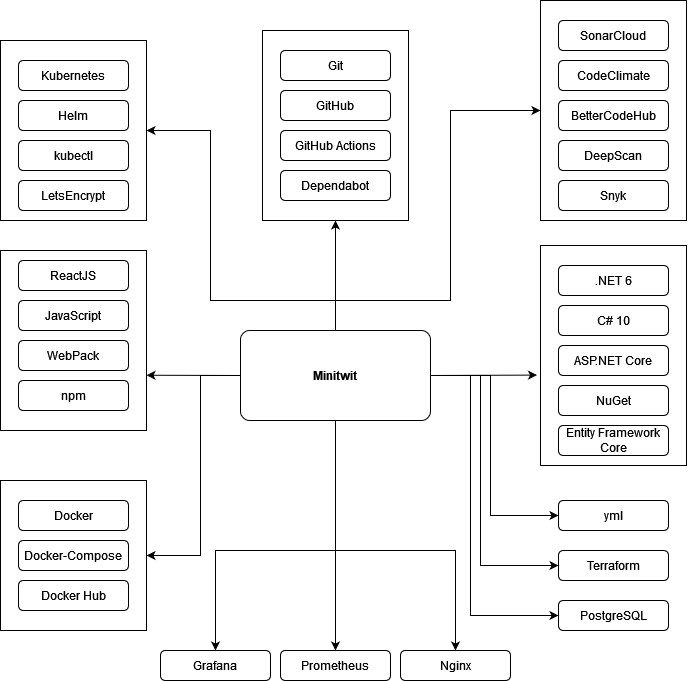
\includegraphics[scale=0.45]{images/DevopsDiagrams-Dependency.drawio(1).png}
    \caption{Technologies \& Tools on which \mini depend. Does not display how these tools and technologies depend on each other.}
    \label{fig:dependencies}
\end{figure}


\subsection{Subsystem Interactions}
\label{subsec:subsystem_interactions}
% - important interactions of subsystems
\begin{figure}[H]
    \centering
    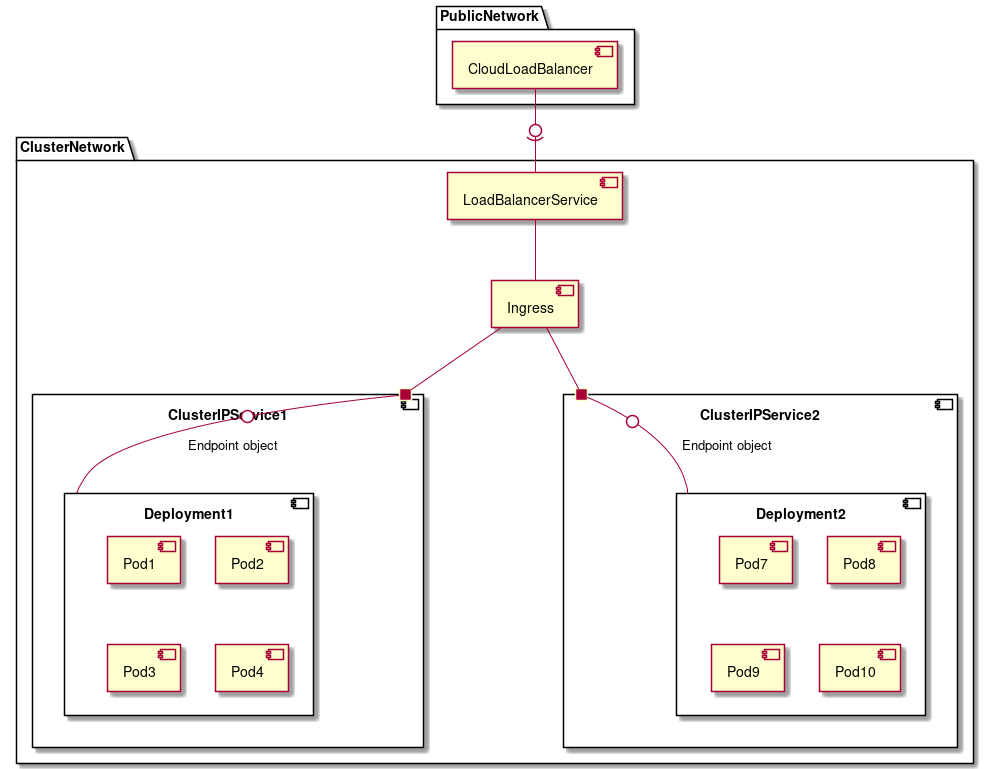
\includegraphics[scale=.4]{images/networking-class.png}
    \caption{Network Component Diagram}
    \label{fig:network_components}
\end{figure}
A notable downside of the microservice architectural pattern is the unreliability of networking interfaces. This makes IP tracking problematic when eliminating single points of failure and providing high service availability.

\subsubsection{The Service Object}
The Kubernetes resource \texttt{Service} provides stable IP addresses, DNS names, and ports through loose coupling to Deployments.
Traffic to microservices is sent to DNS addresses and resolved by the internal cluster DNS to the IP address of the relevant Services, then routed to healthy pods via an \texttt{Endpoint} object that stores a dynamic list of healthy pods matching the Service object's labels \cite{k8sbook}.

\subsubsection{The Cluster Network}
Kubernetes abstracts a cluster of hosts to a single platform (see \textit{Cluster Network} in Figure \ref{fig:network_components}), providing a filesystem, DNS, network, memory sharing, and computational resources. On this network, connected processes and devices are also discoverable, allowing communication between pods given the appropriate IP, though traffic via \texttt{Services} is preferable.

\subsubsection{The LoadBalancer}
The \texttt{Service} object has a few subtypes depending on infrastructure, e.g. a \texttt{LoadBalancerService}.
When a \texttt{LoadBalancerService} is created, Kubernetes provisions a cloud load-balancer (see Figure \ref{fig:network_components}), interfaced by the \texttt{LoadBalancerService}, via the cloud-platform in use. Note that \texttt{LoadBalancerService}, as all Service types, can only interface one Deployment.

\subsubsection{The Ingress Object}
\texttt{Ingress} is a Kubernetes resource allowing access to multiple web applications through a single Service object \cite{k8sbook} and, importantly, providing a reverse proxy to multiple Service objects.

\subsection{System state}
\label{subsec:system_state}
% - Describe the current state of your systems, for example using results of static analysis and quality assessment systems.
% Wait until after cleanup when frontend is merged.
To enable reasoning about our code quality, we have enhanced our \textit{CI} pipeline with static code analysis tools that analyze and rate \mini per their definition of code quality.

\subsubsection{Code Quality, Technical Debt, \& Maintainability}
\label{subsubsec:code_quality}
\mini supports both a simulator API and an API for the frontend resulting in code duplication.\\
\textit{DeepScan} detected no quality issues (see \ref{app:codeAnalDeep}), while \textit{Sonarcloud} suggests a technical debt of 55min and exclusively from the \texttt{Simulation Controller} and infrastructure class, indicating that the simulation \texttt{controller} and \texttt{repository} requires refactoring. In contrast, \textit{Code Climate}(see \ref{app:codeClimate}) scores the technical debt of the system as 2 weeks and finds 17 code smells, highlighting the discrepancy in definitions. However, another factor is Code Climate analyzing the entire repository, while SonarCloud only analyzes the backend (see \ref{fig:codeClimateLangDis}). The frontend contributing heavily to technical debt was expected, as its code quality fell in priority compared to other tasks due to time constraints.  \\
In conclusion, the backend has minimal technical debt. Besides the \texttt{simulation controller} and \texttt{simulation repository} requiring refactoring, code quality is good. However, the technical debt of the frontend hurts the maintainability of the system.

\subsubsection{Vulnerabilities}
2 dedicated security vulnerability scanning tools are used to increase chance of discovering vulnerabilities. Both \textit{Snyk}(see \ref{app:codeAnalSnyk}) and \textit{Dependabot}(see \ref{app:codeAnalDependabot}) finds a vulnerability of high severity stemming from an \textit{npm} dependency, enforcing the fact that it is a known vulnerability. \\
In conclusion, the \mini code base contains two vulnerabilities in the frontend npm modules.


\subsection{License Compatibility}
\label{subsec:license_compatability}
% - Finally, describe briefly, if the license that you have chosen for your project is actually compatible with the licenses of all your direct dependencies.
The initial license chosen was \textit{MIT}, meaning everyone could use and modify the code freely. We are using \textit{ScanCode}\cite{Scancode}, a tool to scan code for licenses, to determine if the license would clash with another license in the imports by scanning the files in the project. 
Through the result we discovered that some of our imports used \textit{Apache License 2.0}\footnote{Apache License 2.0 document\cite{Apache2.0}} and some packages \textit{BSD-3-Clause}\cite{BSD3Clause}, meaning we had to change license.
The new license is Apache 2.0 due to running ScanCode to ensure the license is compatible. The scan seemed to fail on some licenses as it stated them as \textit{Unknown license}. However, since the other licenses encountered are the three mentioned previously, it is likely not a problem. Additionally, when manually searching for the licenses on the imports we use in the frontend, we discovered the majority used MIT license, and one used Apache license 2.0. Therefore the BSD-3-Clause might be some \textit{nodejs} dependency as the license is located in a few development packages alongside Apache license 2.0 and MIT license but in none of the used imports in the code.
%The backend had a license, \textit{IPA Font License} (copy left free font software license -- \textbf{ehh what does this mean?}), this is located in unit test, \textit{xunit}, related \texttt{.dll} files in our \texttt{integration tests} folder in a \texttt{bin/debug} folder. However since this license is only located in the unittests, however since our system is already free this license should not be a problem?
%this IPA Font seems to be something from Japan, idk how much we should include about it.

%Idk if you want to check for yourself if multiple licenses are used in the same file.. but an example is The pack in line 50432-51470 in result.json, which is quite a big file.

%React.router = mit license
%react-router-dom = mit license
%prop-types = mit license
%@mui/material = mit license
%markdown-to-jsx = mit license
%react = mit license
%react-router = mit license
%yup = mit license
%formik = Apache license 2.0

% A description and illustration of the:
% - Double check that for all the weekly tasks (those listed in the schedule) you include the corresponding information.